\chapter{Related work}
\label{chapter:related_work}

In this chapter we will describe the related work in the field of image segmentation using
convolutional neural networks.

\section{Image segmentation}
\label{sec:rw_imgseg}

TODO: will be probably removed

\section{Convolutional neural networks}
\label{sec:cnn_rw}

\subsection{First CNN}
\label{sec:cnn_rw:lecun}

The first convolutional neural network was proposed by LeCun et.
al. in late 1980s.~\cite{bib:lecun1989backpropagation}. Their approach has been
successfully applied to recognition of handwritten digits. Their dataset consisted
of roughly 9298 images, which varied in sizes and styles. Image transformation
was applied to fit them to $16\times16$ pixel area and prepare for feeding to
network. The output consisted of ten neurons, each one computing probability
of given input being digit 0-9. The further development of this project was delayed
because of limited computational capabilities at that time.
Later, Matan et al.~\cite{bib:matan1992multi} extended this project to recognize
strings of digits because previous work was limited to only one-dimensional
input strings. Their approach includes recognizing 5-digit ZIP codes taken from
the U.S Mail using Viterbi encoding.
Since then, CNNs have been ignored by the computer vision community until the mid 2000s
because of lack of computational power.

\subsection{AlexNet}
\label{sec:cnn_rw:alexnet}

The great boom of deep neural networks started after proposing
AlexNet~\cite{bib:krizhevsky2012imagenet}. Krizhevsky et al. competed at the
ImageNet Large Scale Visual Recognition Competition (ILSVRC) in 2012. ImageNet
is a data set of over 15 million labeled high-resolution images with around 22,000
categories. ILSVRC uses just a subset of them which is 1000 categories.

AlexNet consists of 60 million parameters and 650,000 neurons. These neurons
are spread over five convolutional layers and 3 fully connected layers. The
last layer is 1000-way softmax, which produces te distribution over the 1000 class
labels
Convolutional layer filters were of sizes $11\times11$, $5\times5$ and $3\times3$.
Standard activation functions of neuron's input are $f(x) = tanh(x)$ or
$f(x)=(1+e^{-x})^{-1}$. However, in terms of training time with gradient descent,
ReLU (rectified linear unit) activation function is considered much faster. ConvNets
with ReLU train several times faster. To prevent overfitting, data augmentation
and dropout methods were applied.

The full architecture is shown in figure \ref{img:alexnet_architecture}

\begin{figure}[h]
	\centerline{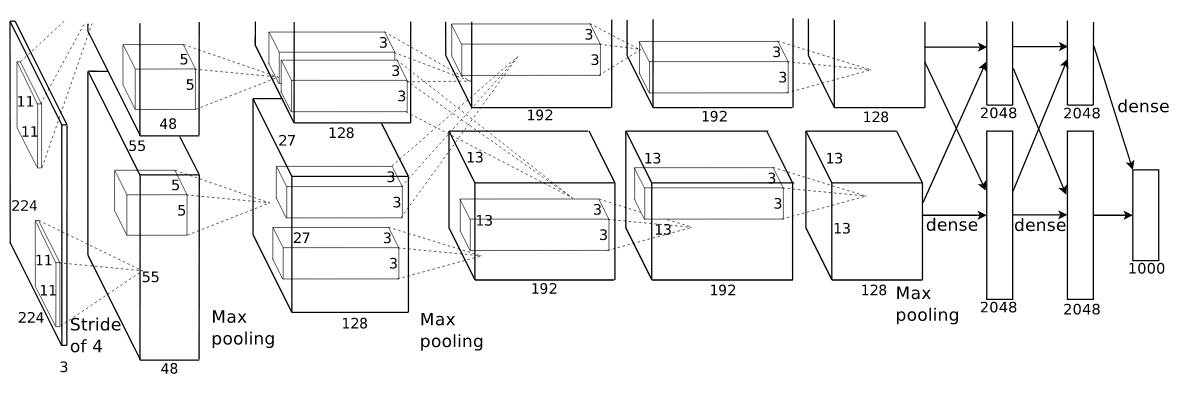
\includegraphics[width=0.9\textwidth]{images/alexnet_architecture.png}}
	\caption[AlexNet architecture]{AlexNet architecture. One GPU runs the
		top part while the other runs the bottom part. They communicate only at
		certain layers. (source \cite{bib:krizhevsky2012imagenet})}
	\label{img:alexnet_architecture}
\end{figure}

AlexNet outperformed previous feature-based methods lowering the error rate down by
40\% compared to hand-engineering approaches. On the test data, they achieved top-1 and
top-5 error rates of 37.5\% and 17.0\%.
Their success was based on using ReLU activation function, local response normalization,
dropout and stochastic gradient descent and in addition usage of GPU during training
and testing process. The network became state-of-the-art in computer vision
classification.

\subsection{GoogLeNet}
\label{sec:cnn_rw:googlenet}

GoogLeNet \cite{bib:szegedy2015going} won ILSVRC competition in 2014. It became new
state-of-the-art CNN, while achieving top-5 error rate of 6.67\% which
was very close to human level performance.

Very impressive fact is that it consisted of 22 layers, but the number of
parameters was reduced to just 4 million (compared to 7 layer AlexNet with 60 million
parameters). Thus, the learning process has sped up .

\subsection{ResNet}
\label{sec:cnn_rw:resnet}

At ILSVRC in 2015, so called ResNet (Residual Neural Network) was introduced
by He et al. \cite{bib:he2016deep}. TODO

\section{Semantic segmentation using CNNs}
\label{sec:semantic_seg_cnn}

Networks for semantic segmentation utilize encoder network followed by decoder network.
Encoder is usually a pre-trained model like VGGNet, ResNet or other classification
network. Architectures mostly differ in decoder. The job of the encoder is to learn
discriminative features at different stages and encode them into high-dimensional feature
vector, whilst
decoder takes this vector and produces semantic segmentation mask.
\cite{bib:semanticsegoveryears}

\subsection{Fully Convolutional Networks for Semantic Segmentation}
\label{sec:semantic_seg_cnn:fcn}

Fully convolutional neural networks proposed by Long et al. \cite{bib:long2015fully}
in 2014
popularized the use of end to end ConvNets for semantic segmentation of natural images.

They adapted contemporary classification networks like AlexNet, VGGnet, and GoogLeNet
and fine-tuned them to segmentation task. The full connected layers of these
classification networks were converted to fully convolutional layers
(see figure \ref{img:transforming_fc_to_conv}).

\begin{figure}[h]
	\centerline{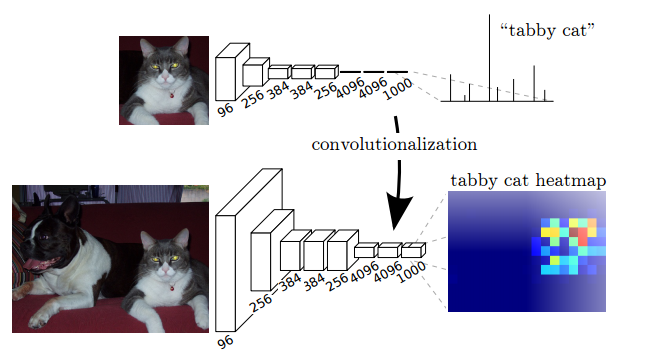
\includegraphics[width=0.9\textwidth]{images/transforming_fc_to_conv.png}}
	\caption[Transformation of fully connected layers into convolutions]{Transformation of fully connected layers into convolutions. (source \cite{bib:long2015fully})}
	\label{img:transforming_fc_to_conv}
\end{figure}

After convolutionalization, they produce class presence heatmaps in low resolution.
Some spatial information is lost because of pooling or strided convolutions,
so it must be upsampled using billinearly initialized deconvolutions and refining
the mask at each stage.

They achieved state-of-the-art segmentation on PASCAL VOC dataset with 20\% relative improvement to 62.2\% mean IU on 2012.

\subsection{SegNet}
\label{sec:semantic_seg_cnn:segnet}

SegNet~\cite{bib:badrinarayanan2015segnet} is another architecture of deep
convolutional neural networks for pixel-wise segmentation. The architecture
of encoder is topologically identical to VGGnet~\cite{bib:simonyan2014very}.
Their contribution is mainly in decoder, which uses pooling indices from encoder
to perform upsampling, thus leaving high frequency details intact in the segmentation.
On the other side, neighboring information is missed when unpooling.
Therefore, the decoder does not have to train upsampling and whole architecture
makes it more memory efficient.

\subsection{U-Net}
\label{sec:semantic_seg_cnn:unet}

U-Net network \cite{bib:ronneberger2015u} got popular in biomedical image analysis.
Since they were forced to train the network with very few data, image augmentation
played a key role in this problem. The dataset the network was trained on contained
only 30 densely annotated images and outperformed best methods on the ISBI challenge
for segmentation of neu-ronal structures in electron microscopic stacks. As discussed in
\cite{bib:ronneberger2015u}, it takes less than a second to segment image on a recent
GPU.

The architecture resembles the character "U", that is why it is called U-Net. On the left
side, there is encoder (or contracting path) which utilizes typical ConvNet architecture.
It contains $3\times3$ convolutions, followed by ReLU and max-pooling operations
for downsampling. Each layer in expanding path consists of upsampling of the feature map,
followed by $2\times2$ convolution, a concatenation of the feature map from the
contracting path and $3\times3$ convolution followed by ReLU. In terms of
data augmentation on microscopical images, they essentially just needed
shift and rotation invariance as well as robustness to deformations and gray value
variation.

This network achieved 92\% mean IU on PhC-U373 beating the second best algorithm
with 83\%. The score achieved on the second dataset called DIC-HeLa was $77.5\%$ mean IU.

\subsection{R-CNN, Fast R-CNN, Faster R-CNN, Mask R-CNN}
\label{sec:semantic_seg_cnn:maskrcnn}

Mask R-CNN published by He et al.~\cite{bib:he2017mask} in 2017 builds on previous
object detection works R-CNN~\cite{bib:girshick2014rich},
Fast R-CNN~\cite{bib:girshick2015fast} and Faster R-CNN~\cite{bib:ren2015faster}.

The original R-CNN is a four step process:
\begin{enumerate}
	\item Input an image
	\item Extract regions potentially containing objects (region proposals)
	\item Compute features from each region proposal using pre-trained CNN
	\item Classify each proposal using linear SVM
\end{enumerate}

The problem of R-CNN is that it is enormously slow. Also, the model does not learn to
localize objects using deep CNN. The contribution of Fast R-CNN was region of
interest (ROI) pooling module, which essentially extracted fixed-size window
from feature map. The network became end-to-end trainable but the performance
was dependent on selective search and therefore suffered at prediction time.

To make it even faster, Ren et al. proposed Faster R-CNN. It utilizes so called
Region Proposal Network (RPN), which alleviates the need for selective search. Regions
of interests are generated and top $N$ are kept according to their objectness
score. In the original paper $N$ is set to 2000.
Faster
R-CNN architecture is capable of running at 7-10 FPS, which is a huge step towards
real-time object detection with deep networks.

Mask R-CNN has been published with two major contributions:
\begin{enumerate}
	\item Replaced ROI pooling module with more accurate ROI align module
	\item Inserted an additional branch out of the ROI align module to produce 
	mask of the object
\end{enumerate}

The network is therefore able to produce three outputs - bounding box of the object,
its mask and label.

\subsection{MultiNet}
\label{sec:semantic_seg_cnn:multinet}

In 2018, Teichmann et al. \cite{bib:teichmann2018multinet} published an interesting
paper on road segmentation. In their approach they efficiently perform
classification, detection and semantic segmentation simultaneously.

Model architecture is traditional encoder-decoder. The difference is that there
is just one encoder producing rich features shared among all the tasks. These features
are then utilized by task specific decoders.
Encoder's weights are pre-trained on ImageNet classification data. They performed
experiments on VGG16 and ResNet architectures. The first one is called VGG-pool5
as it discards all fully-connected layers from VGG and pool5 is the last layer.
The second implementation is called VGG-fc7 because it only discards the final softmax
layer. Layers fc6 and fc7 are replaced by $1\times1$ convolutions. This allows the
network to process images of arbitrary size. For ResNet they implemented 50 and 101
layer version of the network and discarded fully-connected softmax.

Decoder architecture follows the FCN architecture \cite{bib:long2015fully}.
Segmentation is applied to input
downsampled by encoder to size $39\times12$ using $1\times1$ convolution layer. Then,
it is upsampled using three transposed convolution layers.

MultiNet's training strategy is fine-tuning. The encoder is trained to perform
classification on ILSVRC2012 dataset. But in practice, this step is omitted and
encoder is initialized using pre-trained weights of networks they are using.
The second step is dedicated to replacing fully connected layers with
convolution ones.

Authors evaluated the proposed model on KITTI dataset, which contains images
from various street situations captured from a moving platform in the city.
The segmentation module reached MaxF1 score of 94.88\% with average precision of
93.71\% beating all other submissions. Moreover, the speed of prediction is 42.48ms
for all tasks, which is very efficient for real-time predictions.

According to their comparison of VGG and ResNet they observed that both ResNets
outperformed VGGs. But we can see there is a trade-off because VGGs are faster.
\\
\\


TODO: Jariabka, Suppa - CNN smely zajac 

TODO: zmensovanie neuroniek - nejake clanky - mozno


\section{Active learning}
\label{sec:active_learning_rw}

TODO: active learning clanky